\documentclass[border=10pt, tikz]{standalone}
\usepackage{amsmath}
\usepackage{amssymb}
\usepackage{ctex}
\usepackage{xcolor}
\usepackage{tikz}
\usetikzlibrary{matrix, calc, positioning}
\usetikzlibrary{arrows.meta}

\begin{document}
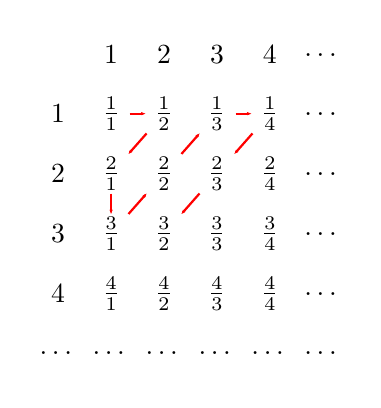
\begin{tikzpicture}
	% 定义矩阵
	\matrix (m) [matrix of nodes, nodes={minimum size=1.3em, inner sep=1pt, anchor=center},
		column sep=-0.5\pgflinewidth+4pt, row sep=-0.5\pgflinewidth+8pt]
	{
		~      & 1             & 2             & 3             & 4             & \ldots \\
		1      & $\frac{1}{1}$ & $\frac{1}{2}$ & $\frac{1}{3}$ & $\frac{1}{4}$ & \ldots \\
		2      & $\frac{2}{1}$ & $\frac{2}{2}$ & $\frac{2}{3}$ & $\frac{2}{4}$ & \ldots \\
		3      & $\frac{3}{1}$ & $\frac{3}{2}$ & $\frac{3}{3}$ & $\frac{3}{4}$ & \ldots \\
		4      & $\frac{4}{1}$ & $\frac{4}{2}$ & $\frac{4}{3}$ & $\frac{4}{4}$ & \ldots \\
		\ldots & \ldots        & \ldots        & \ldots        & \ldots        & \ldots \\
	};

	% 绘制折线
	\tikzset{
	arrow/.style = {arrows = {-Stealth[length=3pt, inset=2pt]}, thick, red}
	}

	\draw (m-2-2) edge [arrow] (m-2-3);
	\draw (m-2-3) edge [arrow] (m-3-2);
	\draw (m-3-2) edge [arrow] (m-4-2);
	\draw (m-4-2) edge [arrow] (m-3-3);
	\draw (m-3-3) edge [arrow] (m-2-4);
	\draw (m-2-4) edge [arrow] (m-2-5);
	\draw (m-2-5) edge [arrow] (m-3-4);
	\draw (m-3-4) edge [arrow] (m-4-3);

\end{tikzpicture}
\end{document}
